\documentclass{article}
\usepackage[utf8]{inputenc}
\usepackage{graphicx}
\usepackage{makeidx}
\usepackage{geometry}
\usepackage{float}
\usepackage{indentfirst}


\renewcommand{\contentsname}{Índice}
\geometry{a4paper,total = {150mm,250mm},left = {30mm}, top = {30mm}}
\makeindex
\graphicspath{ {./imagens/} }
\begin{document}
\begin{capa}
	\begin{center}
	\vspace*{1.0cm}
	\huge{Universidade do Minho}\\
	[1.0cm]
	
\includegraphics{logo.jpg}\\
	[1.5cm]
	\huge{\textbf{Redes de Computadores}}\\
	[0.5cm]
	\textsc{RC-TP2}\\
	\textsc{\normalsize{Mestrado Integrado em Engenharia Informática}}\\
	\textsc{\normalsize{3º Ano}}\\
	\textsc{\normalsize{Grupo 61}}\\
	[12.0cm]
	\end{center}
	\begin{flushleft}
	\textsc{Renato André Araújo Azevedo \textbf{\hspace*{130pt} A89547}}\\
	\textsc{Gonçalo Costa de Almeida \textbf{\hspace*{151pt} A88292}}\\
	\textsc{Maria Sofia Martinho Gonçalves Jordão Marques \textbf{\hspace*{30pt} A87963}}\\
	\end{flushleft}
\end{capa}

\newpage
\tableofcontents
\newpage

\section{Introdução}
	No âmbito da cadeira de Redes Computadores foi-nos proposta a elaboração de um trabalho composto por duas partes que terá como principal objetivo  o estudo do Internet Protocol (IP) nas suas principais vertentes, nomeadamente:  estudo do formato de um pacote ou datagrama IP, fragmentação de pacotes IP, endereçamento IP e  encaminhamento IP.\par
        Na primeira parte deste projeto será realizado o registo de datagramas IP  estes serão analisados os vários campos de um datagrama IP e detalhado o processo de fragmentação realizado pelo IP. Na segunda parte deste projeto continua-se o estudo do protocolo IPv4 com ênfase no endereçamento e encaminhamento IP. Serão também apresentadas algumas das técnicas mais relevantes que foram propostas para aumentar a escalabilidade do protocolo IP, apaziguar a exaustão dos endereços IPv4 e também reduzir os recursos de memoria necessários nos routers para manter as tabelas de encaminhamento.\par
	Esperamos, com este trabalho, atingir os objetivos definidos pelo docente. \\

\section{Parte 1}
\subsection{Ex1}
\textbf{Prepare uma topologia CORE para verificar o comportamento do traceroute. Ligue um host (pc) Cliente1 a um router R2; o router R2 a um router R3, que por sua vez, se liga a um host (servidor) Servidor1. (Note que pode não existir conectividade IP imediata entre o Cliente1 e o Servidor1 até que o anúncio de rotas estabilize). Ajuste o nome dos equipamentos atribuídos por defeito para a topologia do enunciado.}\\\par

\begin{figure}[h]
	\centering
	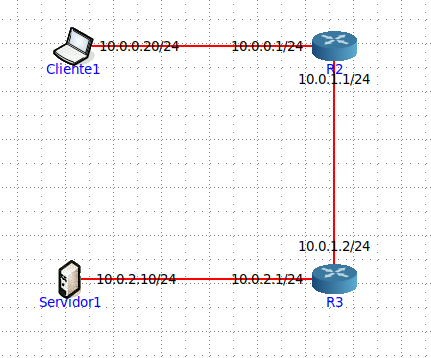
\includegraphics[scale = 0.8]{topologia-ex1.png}
	\caption{Topologia Core}
\end{figure}
\subsubsection{Alínea a}
\textbf{Active o wireshark ou o tcpdump no Cliente1. Numa shell do Cliente1, execute o comando traceroute -I para o endereço IP do Servidor1.}		
\begin{figure}[h]
	\centering
	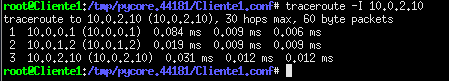
\includegraphics[scale = 0.8]{traceroute-ex1.png}
	\caption{Shell com o traceroute -I}
\end{figure}
\newpage
\subsubsection{Alínea b}	
\textbf{Registe e analise o tráfego ICMP enviado pelo Cliente1 e o tráfego ICMP recebido como resposta. Comente os resultados face ao comportamento esperado.}\\\par
\begin{figure}[h]
	\centering
	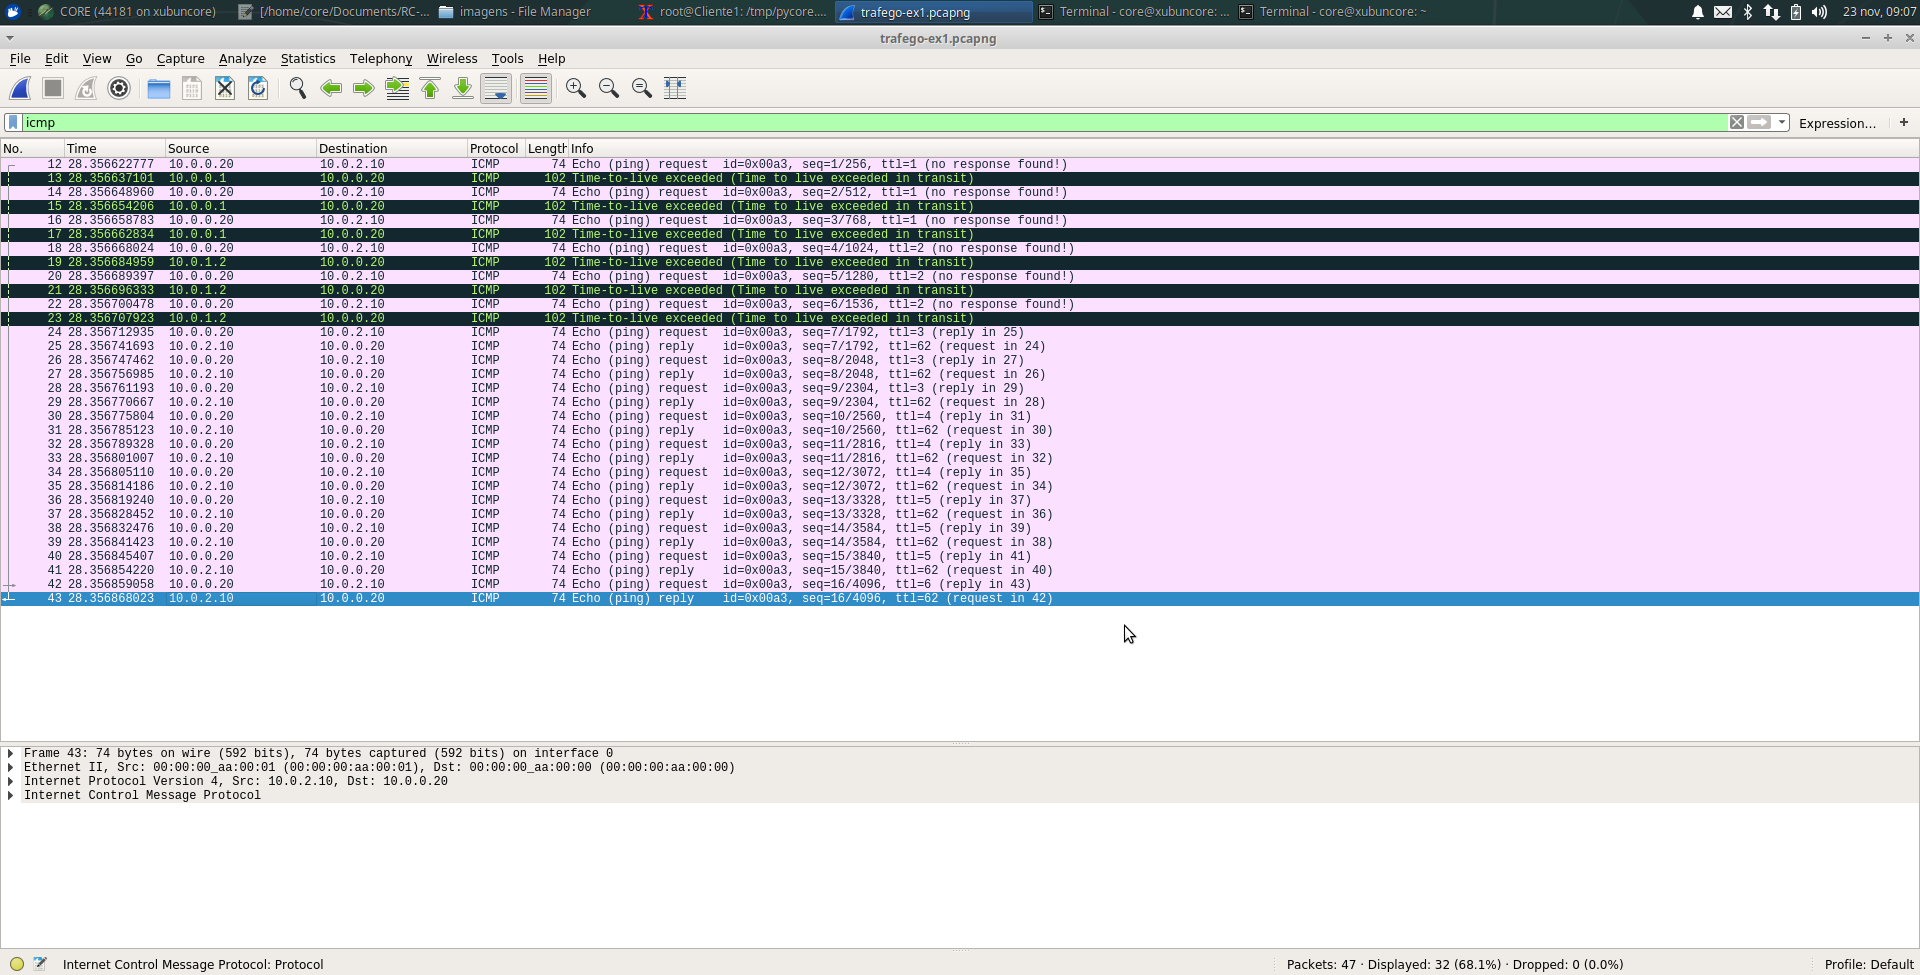
\includegraphics[scale = 0.2]{trafego-ex1.png}
	\caption{Trafego do wireshark}
\end{figure}	
Em cada salto que a mensagem efetua, o TTL é decrementado em 1. Desta forma será de esperar que enquanto o TTL não for 3, ou seja, igual ao número de saltos, vamos recever respostas TTL exceeded. Na prática, o cliente envia 3 pings com TTL = 1 para o R1, onde o R1 responde com TTL exceeded, tal como seria de esperar, uma vez que o TTL foi decrementado pelo router R1, chegando a 0. Depois o mesmo acontece para o R2, uma vez que o router R1 reduziu o TTL para 1. Por fim, quando TTL = 3, a mensagem consegue chegar  ao Servidor1, obtendo uma resposta.\\

\subsubsection{Alínea c}
\textbf{Qual deve ser o valor inicial mínimo do campo TTL para alcançar o Servidor1? Verifique na prática que a sua resposta está correta.}\\\par
\begin{figure}[h]
	\centering
	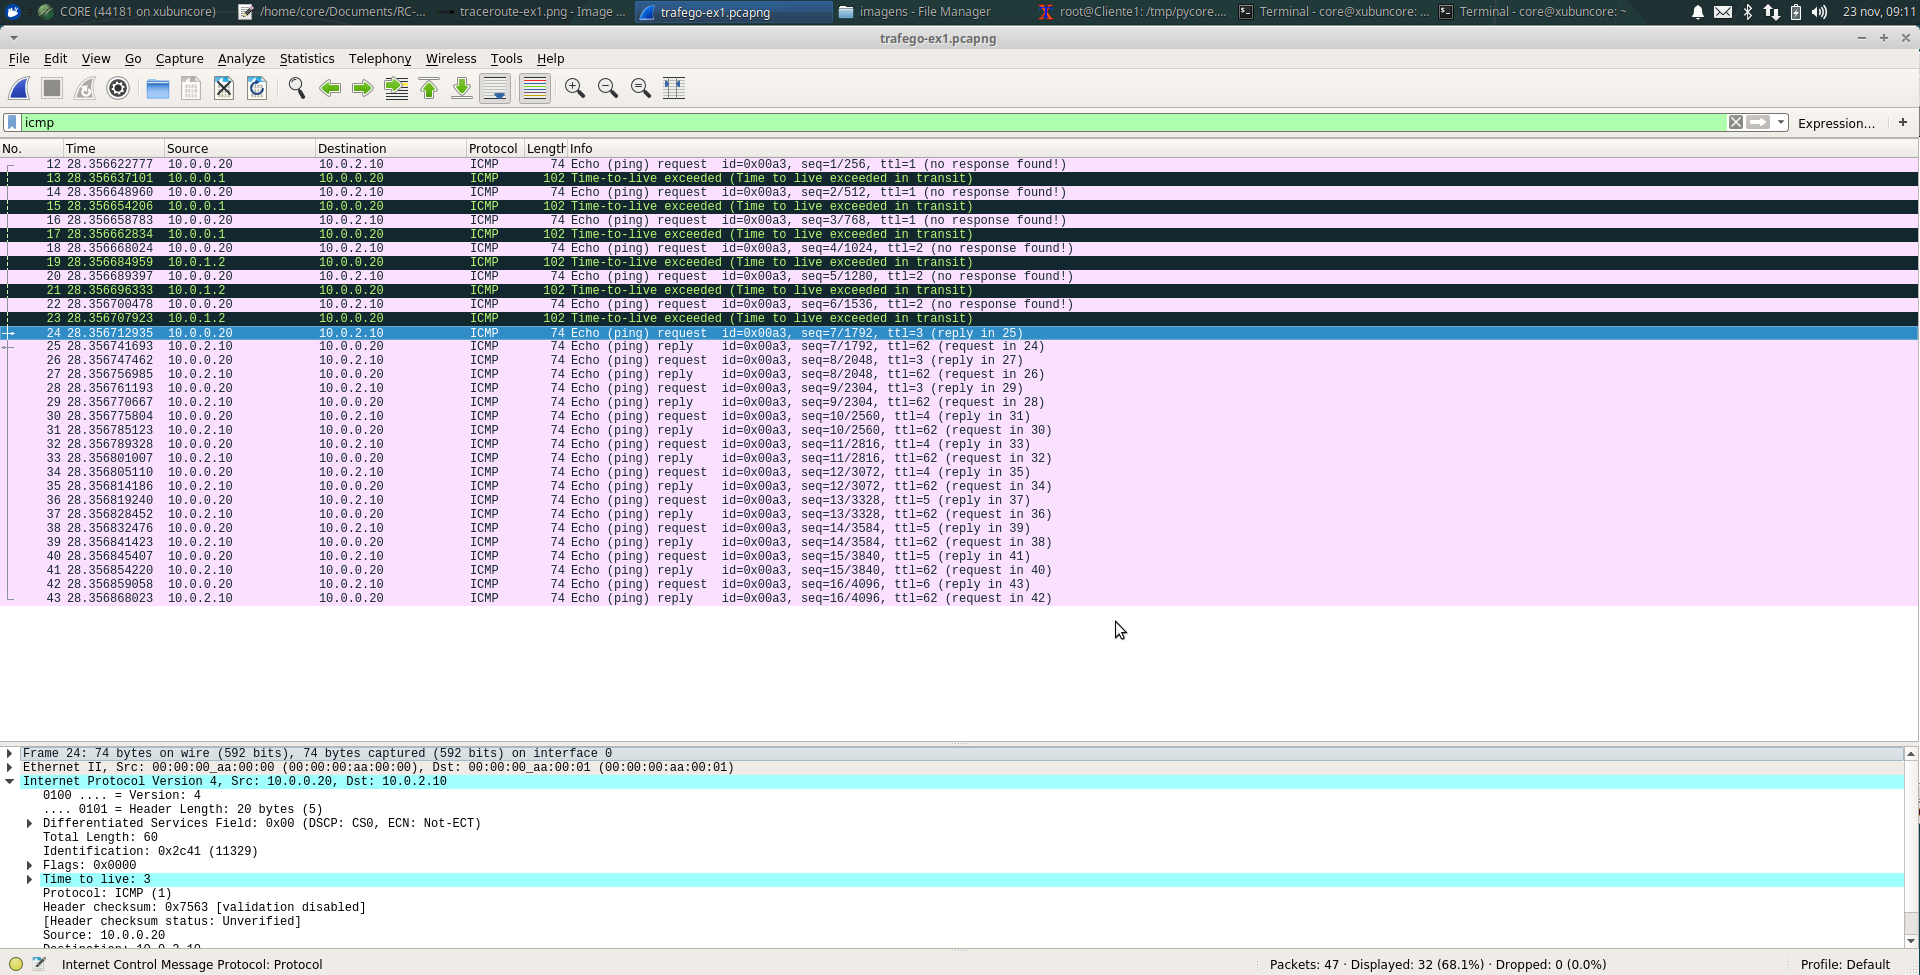
\includegraphics[scale = 0.2]{ttl-ex1.png}
	\caption{TTL ex 1}
\end{figure}
Para alcançar o servidor1, o TTL esperado seria de 3, uma vez que se encontra a 3 saltos do cliente1. O que se verifica na prática, tal como se observa na imagem anterior, onde deixamos de recever TTL exceeded quando o TTL chega a 3.

\subsubsection{Alínea d}	
\textbf{Calcule o valor médio do tempo de ida-e-volta (Round-TripTime) obtido?}\\\par
Os tempos obtidos foram:

\begin{itemize}
	\item Para o R2: 0.084 ms, 0.009 ms, 0.006 ms, com uma média de 0.033 ms
	\item Para o R3: 0.019 ms, 0.009 ms, 0.009 ms, com uma média de 0.012 ms
	\item Para o Servidor1: 0.031 ms, 0.012 ms, 0.012 ms, com uma média de 0.018 ms
\end{itemize}

\subsection{Ex2}
\textbf{Selecione a primeira mensagem ICMP capturada (referente a (i) tamanho por defeito) e centre a análise no nível protocolar IP (expanda o tab correspondente na janela de detalhe do wireshark). Através da análise do cabeçalho IP diga:}

\subsubsection{Alinea a}
\textbf{Qual é o endereço IP da interface ativa do seu computador?} \\\par
O valor do IP da interface do computador é 172.26.47.154.\\

\subsubsection{Alinea b}
\textbf{Qual é o valor do campo protocolo? O que identifica?} \\\par
Como podemos observar na imagem, o campo do protocolo tem valor 1, o que corresponde ao protocolo ICMP. \\

\begin{figure}[h]
	\centering
	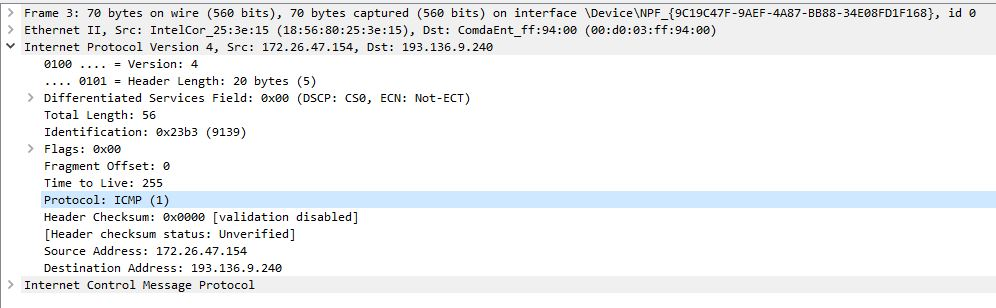
\includegraphics[scale = 0.5]{valor-campo-protocolo.JPG}
	\caption{Valor do campo protocolo}
\end{figure}

\subsubsection{Alinea c}
\textbf{Quantos bytes tem o cabeçalho IP(v4)? Quantos bytes tem o campo de dados (payload) do datagrama? Como se calcula o tamanho do payload?} \\\par
O cabeçalho IP(v4) possui 20 bytes, pelo \textit{Header Length}. Como o \textit{Total Length} possui 56 bytes, então o {payload} deverá ter 36 bytes, uma vez que o \textit{Total Length} = \textit{Header Length} + \textit{payload}.\\

\begin{figure}[h]
	\centering
	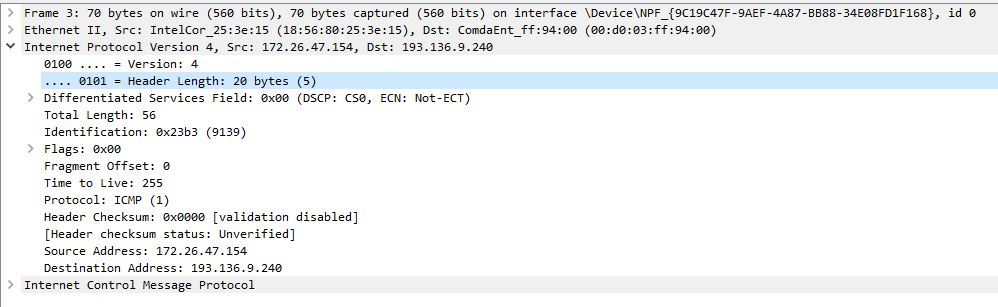
\includegraphics[scale = 0.5]{calculo-payload.JPG}
	\caption{Calculo do payload}
\end{figure}

\subsubsection{Alinea d}
\textbf{O datagrama IP foi fragmentado? Justifique.} \\\par
Como \textit{Flags} = 0s, \textit{Fragment Offset} = 0, podemos concluir que a mensagem não foi fragmentada, uma vez que o \textit{Fragment Offset} a zero indica que seria o primeiro fragmento, e a flag \textit{More fragments} a zero indica que não existem mais fragmentos.\\\par

\begin{figure}[h]
	\centering
	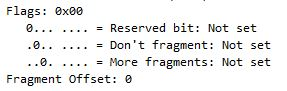
\includegraphics[scale = 0.8]{flags.JPG}
	\caption{Flags}
\end{figure}

\subsubsection{Alinea e}
\textbf{Ordene os pacotes capturados de acordo com o endereço IP fonte (e.g., selecionando o cabeçalho da coluna Source), e analise a sequência de tráfego ICMP gerado a partir do endereço IP atribuído à interface da sua máquina. Para a sequência de mensagens ICMP enviadas pelo seu computador, indique que campos do cabeçalho IP variam de pacote para pacote.} \\\par
Os valores que se alteram são o \texit{identification}, e o \textit{time to live}.\\

\begin{figure}[h]
	\centering
	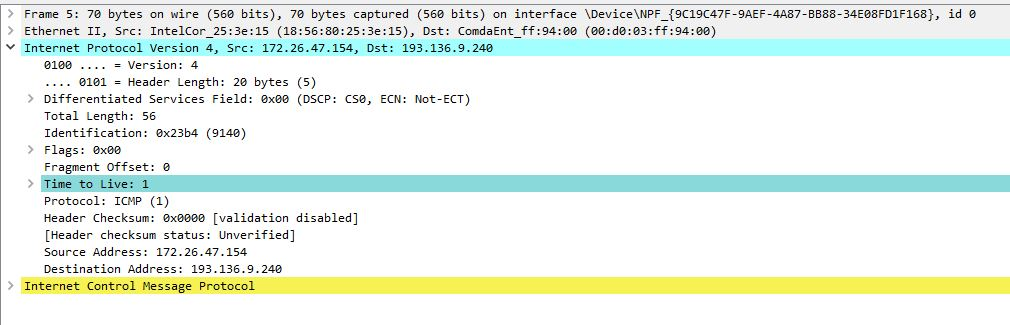
\includegraphics[scale = 0.5]{valores-variam-1.JPG}
	\caption{Variação dos valores 1}
\end{figure}

\begin{figure}[h]
	\centering
	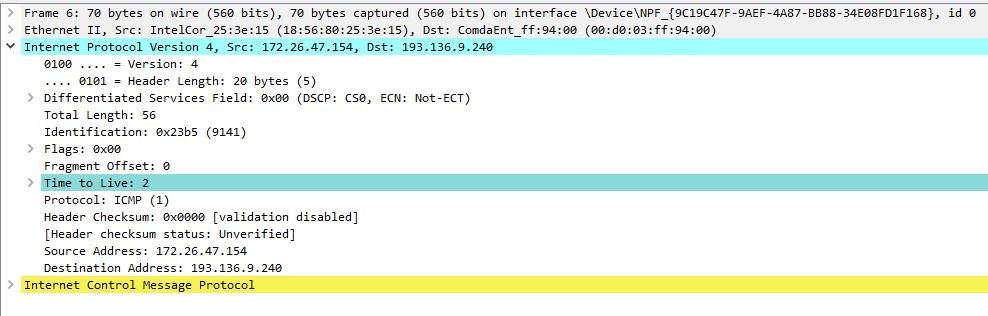
\includegraphics[scale = 0.5]{valores-variam-2.JPG}
	\caption{Variação dos valores 2}
\end{figure}

\newpage

\subsubsection{Alinea f}
\textbf{Observa algum padrão nos valores do campo de Identificação do datagrama IP e TTL?} \\\par
Em cada datagrama temos que $\textit{identification}_{i+1}$ = 1 + $\textit{identification}_i$.\par
Em cada datagrama temos que o valor de $TTL_{i+1}$ será:
\begin{itemize}
	\item 1 se $TTL_i$ = 255
	\item 255 se $TTL_i$ = 3
	\item $TTL_i$ + 1 caso contrário
\end{itemize}\par

\begin{figure}[h]
	\centering
	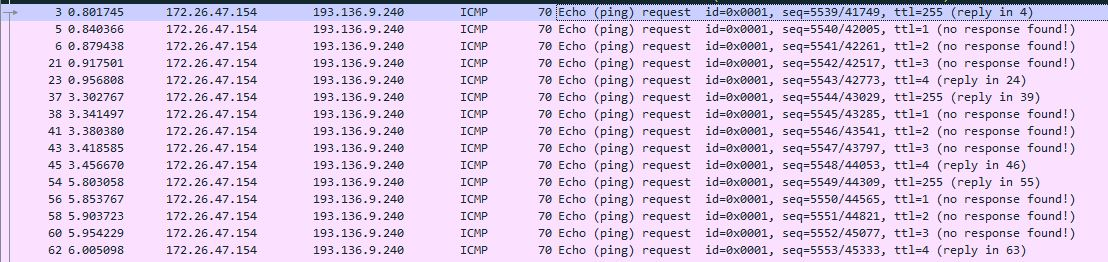
\includegraphics[scale = 0.5]{valores-padroes.JPG}
	\caption{Valores do TTL}
\end{figure}

\subsubsection{Alinea g}
\textbf{Ordene o tráfego capturado por endereço destino e encontre a série de respostas ICMP TTL exceeded enviadas ao seu computador. Qual é o valor do campo TTL? Esse valor permanece constante para todas as mensagens de resposta ICMP TTL exceeded enviados ao seu host? Porquê?} \\\par
Nas primeiras respostas ICMP TTL exceeded temos um valor TTL inicial de 255 que vai diminuindo até 253. Isto acontece porque a mensagem faz 3 saltos até ao destino, onde o TTL é decrementado em 1 por cada salto. Na primeira mensagem recebemos o TTL máximo de 255, uma vez que a mensagem só chegou até ao primeiro router, não sendo decrementado por nenhum router. Depois, na segunda mensagem, o TTL será 254, por ter sido decrementado em 1 pelo router intermédio. Por fim será de 253, uma vez que passou por dois routers intermédios, tendo sido decrementado duas vezes.\\

\begin{figure}[h]
	\centering
	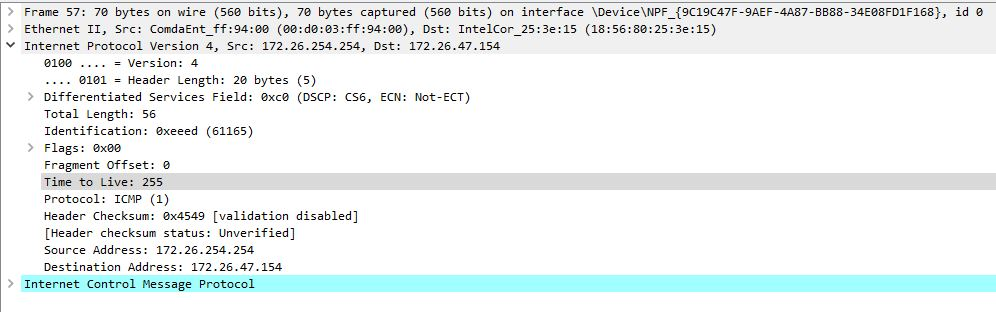
\includegraphics[scale = 0.5]{ttl-2g2.JPG}
	\caption{Primeiro valor TTL}
\end{figure}

\newpage

\begin{figure}[h]
	\centering
	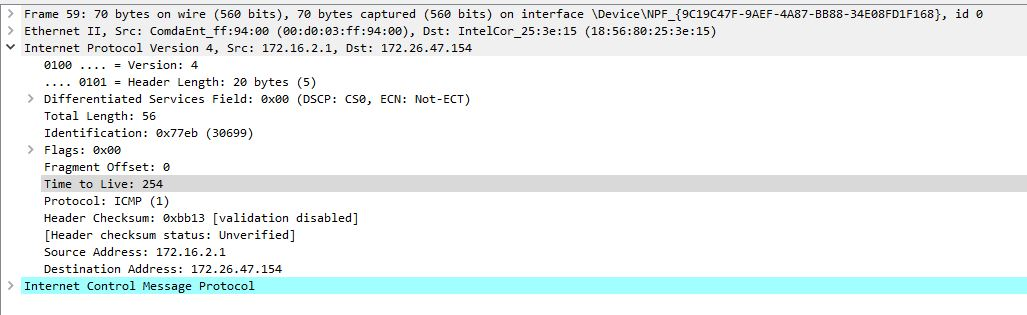
\includegraphics[scale = 0.5]{ttl-2g.JPG}
	\caption{Segundo valor TTL}
\end{figure}

\begin{figure}[h]
	\centering
	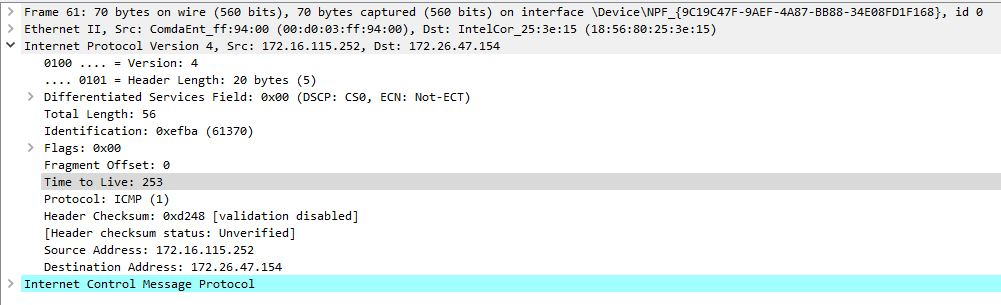
\includegraphics[scale = 0.5]{ttl-2g3.JPG}
	\caption{Terceiro valor TTL}
\end{figure}

\subsection{Ex3}
\textbf{Pretende-se agora analisar a fragmentação de pacotes IP. Reponha a ordem do tráfego capturado usando a coluna do tempode captura. Observe o tráfego depois do tamanho de pacote ter sido definido para 32XX bytes.}

\subsubsection{Alinea a}
\textbf{Localize a primeira mensagem ICMP. Porque é que houve necessidade de fragmentar o pacote inicial?} \\\par
A mensagem teve de ser fragmentada, uma vez que a quantidade de bytes que se pretende eviar é superior ao máximo definido, sendo fragmentada em 2 mensagens com 1514 bytes e 1 mensagem de 315 bytes.\\

\newpage

\begin{figure}[h]
	\centering
	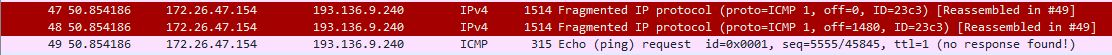
\includegraphics[scale = 0.5]{fragmentos.JPG}
	\caption{Mensagem fragmentada}
\end{figure}

\subsubsection{Alinea b}
\textbf{Imprima o primeiro fragmento do datagrama IP segmentado. Que informação no cabeçalho indica que o datagrama foi fragmentado? Que informação no cabeçalho IP indica que se trata do primeiro fragmento? Qual é o tamanho deste datagrama IP?} \\\par
A flag \textit{More fragments} permite verificar se o texto foi fragmentado. Como esta como Set, podemos confirmar a existencia de mais fragmentos. Para saber que se trata do primeiro fragmento, basta olhar para o campo \textit{Fragment Offset}, e como este está a 0, podemos saber que este é o primeiro fragmento. Como \textit{Total Length} = 1500, sabemos que o tamanho da mensagem é de 1500 bytes, sendo 20 para o cabeçalho e 1480 para o payload).\\

\begin{figure}[h]
	\centering
	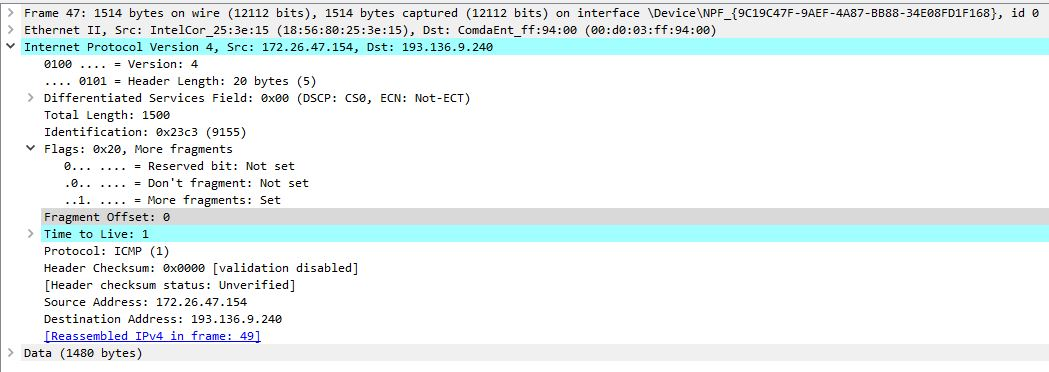
\includegraphics[scale = 0.5]{primeiro-fragmento.JPG}
	\caption{Primeiro fragmento do datagrama IP}
\end{figure}

\subsubsection{Alinea c}
\textbf{Imprima o segundo fragmento do datagrama IP original. Que informação do cabeçalho IP indica que não se trata do 1ºfragmento? Há mais fragmentos? O que nos permite afirmar isso?} \\\par
Como o \textit{Fragment Offset} = 1480, podemos concluir que esta se trata da segunda mensagem, já que a primeira tem um \textit{Total Length} de 1500, onde 1480 são para o \textit{payload}, sendo esse o \textit{Offset} da segunda mensagem.\\

\begin{figure}[h]
	\centering
	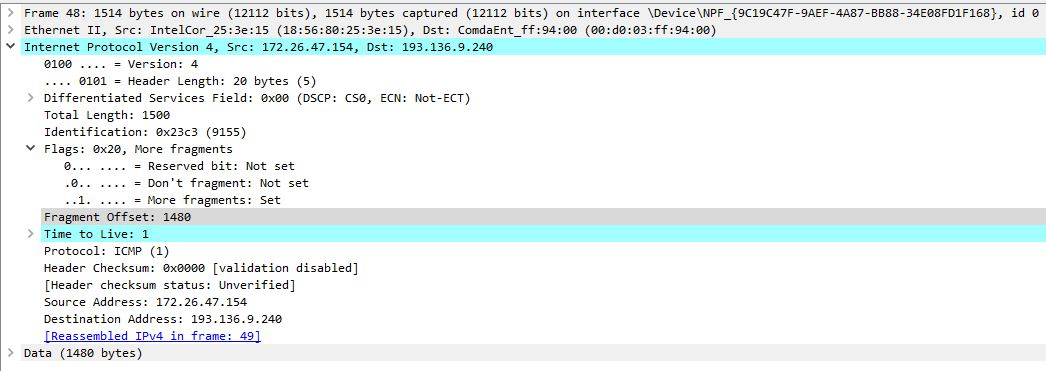
\includegraphics[scale = 0.5]{segundo-fragmento.JPG}
	\caption{Segundo fragmento do datagrama IP}
\end{figure}

\subsubsection{Alinea d}
\textbf{Quantos fragmentos foram criados a partir do datagrama original? Como se detecta o último fragmento correspondente ao datagrama original?} \\\par
Foram criados 3 fragmentos, podendo identificar o último através da flag \textit{More fragments}, que está \textif{Not set}, o que significa que não existem mais fragmentos. Sendo assim podemos identificar 3 fragmentos da mensagem, como vimos nas imagens anteriores.\\

\begin{figure}[h]
	\centering
	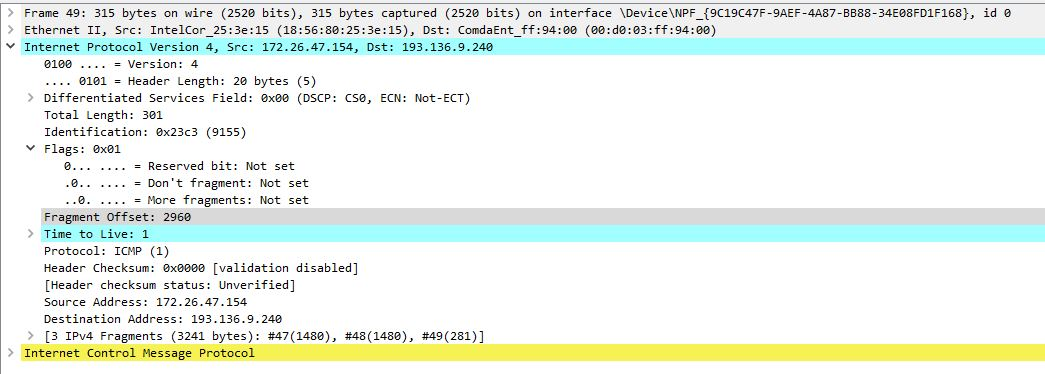
\includegraphics[scale = 0.5]{ultimo-fragmento.JPG}
	\caption{Ultimo fragmento do datagrama IP}
\end{figure}

\subsubsection{Alinea e}
\textbf{Indique, resumindo, os campos que mudam no cabeçalho IP entre os diferentes fragmentos, e explique a forma como essa informação permite reconstruir o datagrama original.} \\\par
Os campos que se alteram no cabeçalho IP dos 3 fragmentos são \textit{More fragments} e o \textit{Fragment Offset}. Para reconstruir o datagrama original, devemos organizar os fragmentos por ordem crescente do offset, tendo em consideração que o ultimo fragmento será o que tiver a flag \textit{More fragments} a zero, visto que esta indica que não existem mais fragmentos desse datagrama.\\

\newpage

\section{Parte 2}

\subsection{Ex1}
\textbf{Atenda aos endereços IP atribuídos automaticamente pelo CORE aos diversos equipamentos da topologia.}
\subsubsection{Alinea a}
\textbf{Indique que endereços IP e máscaras de rede foram atribuídos pelo CORE a cada equipamento. Para simplificar, pode incluir uma imagem que ilustre de forma clara a topologia definida e o endereçamento usado.}\\\par

\begin{figure}[h]
	\centering
	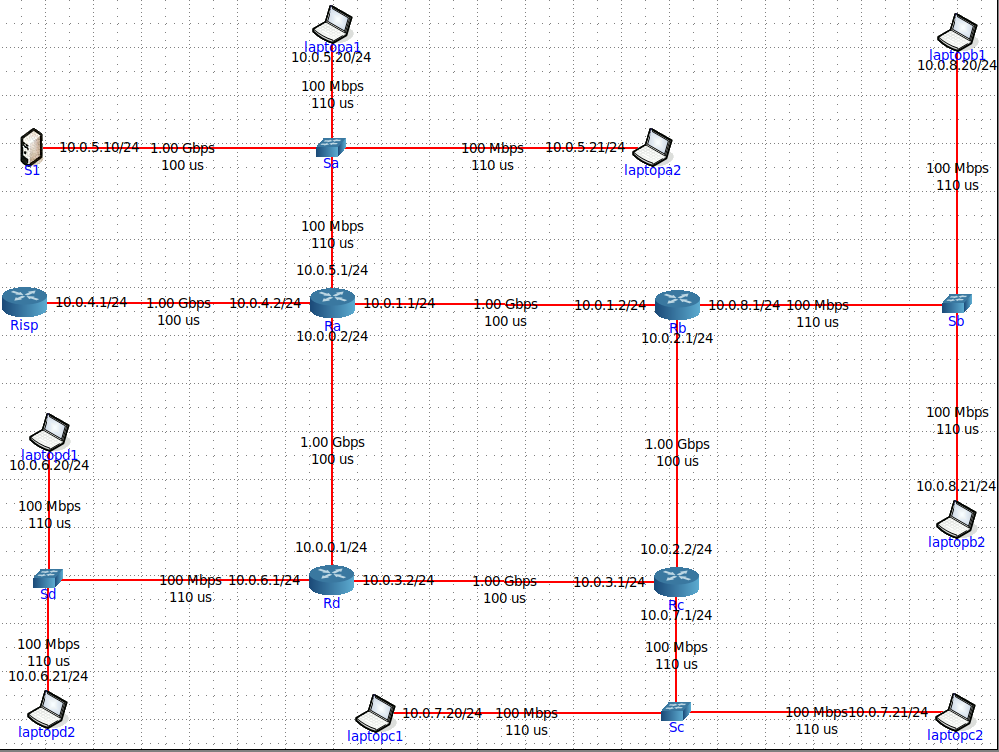
\includegraphics[scale = 0.4]{rede-tp2-ex1.png}
	\caption{Topologia da rede}
\end{figure}

\subsubsection{Alinea b}
\textbf{Tratam-se de endereços públicos ou privados? Porquê?}\\\par
Os endereços privados encontram-se em 3 intervalos:	
\begin{itemize}
	\item bloco 192.168.00 - 192.168.255.255 / 16
	\item bloco 172.16.0.0 - 172.31.255.255 / 12
	\item bloco 10.0.0.0 - 10.255.255.255 / 6
\end{itemize}\par
Como podemos observar, os ips atribuidos pelo core encontram-se na terceira gama, o que significa que são IPs privados.\\

\subsubsection{Alinea c}
\textbf{Porque razão não é atribuído um endereço IP aos switches?}\\\par
Os switches não tem ip uma vez que apenas trabalham na camada pysical e link, ao contrário dos routers que por sua vez já trabalham na camada do network, dai serem lhes atribuido ips. \\

\subsubsection{Alinea d}
\textbf{Usando o comando ping certifique-se que existe conectividade IP entre os laptops dos vários departamentose o servidor do departamento A (basta certificar-se   daconectividade de um laptop por departamento).}\\\par
Como mostram as imagens, podemos concluir que existe conexão entre os computadores dos departamentos e o servidor S_1.\\

\begin{figure}[h]
	\centering
	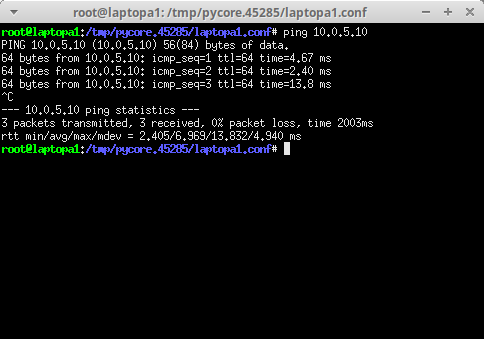
\includegraphics[scale = 0.6]{conectividade-redea-ex1.png}
	\caption{Conctividade no departamento A}
\end{figure}

\begin{figure}[h]
	\centering
	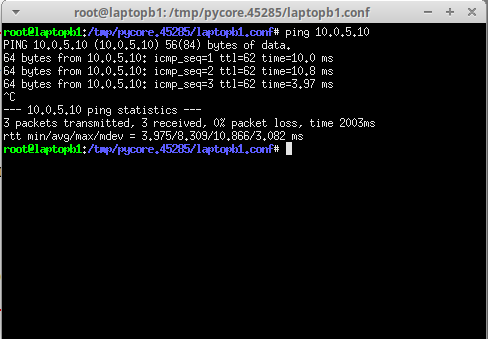
\includegraphics[scale = 0.6]{conectividade-redeb-ex1.png}
	\caption{Conctividade no departamento B}
\end{figure}

\begin{figure}[h]
	\centering
	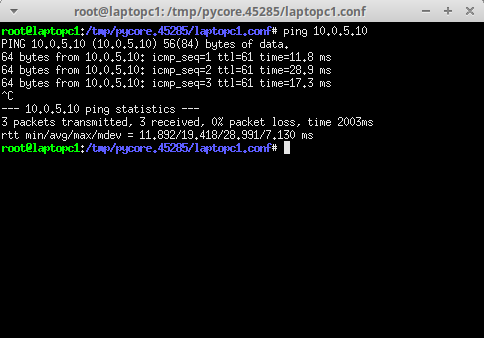
\includegraphics[scale = 0.6]{conectividade-redec-ex1.png}
	\caption{Conctividade no departamento C}
\end{figure}

\begin{figure}[h]
	\centering
	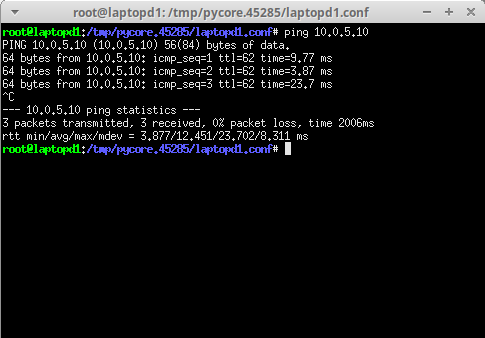
\includegraphics[scale = 0.6]{conectividade-reded-ex1.png}
	\caption{Conctividade no departamento D}
\end{figure}

\subsubsection{Alinea e}
\textbf{Verifique se existe conectividade IP do router de acesso RISP para o servidor S1.}\\\par
Como podemos ver na imagem, existe conexão entre o router de acesso $R_{isp}$ e o servidor S_1.\\

\newpage

\begin{figure}[h]
	\centering
	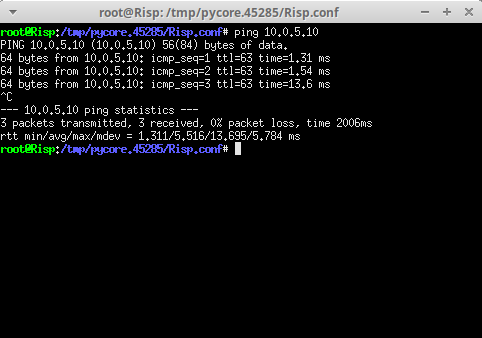
\includegraphics[scale = 0.6]{conectividade-risp-ex1.png}
	\caption{Conctividade no router ISP}
\end{figure}

\subsection{Ex2}
\textbf{Para o router e um laptop do departamento C:}
\subsubsection{Alinea a}
\textbf{Execute o comando netstat –rn por forma a poder consultar a tabela de encaminhamento unicast (IPv4). Inclua no seu relatório as tabelas de encaminhamento obtidas; interpreteas várias entradas de cada tabela. Se necessário, consulte o manual respetivo (man netstat).}\\\par

Nas tabelas de encaminhamento, a coluna \textit{Destination} representa o IP do destino da mensagem. Já a coluna \textit{Gateway} representa o IP do proximo nodo onde será enviada a mensagem. Por fim, a coluna \textit{Genmask} representa a máscara aplicada ao IP destino. 

\begin{figure}[h]
	\centering
	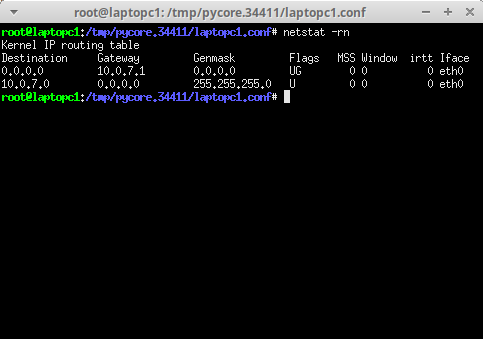
\includegraphics[scale = 0.6]{tabela-enderecamento-laptop1.png}
	\caption{Tabela de encaminhamento de um laptop}
\end{figure}

A primeira entrada na tabela representa a rota por defeito, encaminhando a mensagem para o router C. Já a segunda entrada, representa a rota com destino para a rede local.

\newpage

\begin{figure}[h]
	\centering
	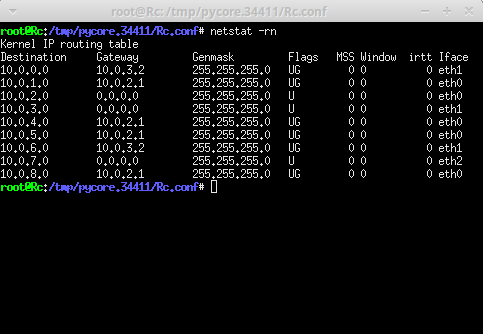
\includegraphics[scale = 0.6]{tabela-enderecamento-Rc.png}
	\caption{Tabela de encaminhamento do router C}
\end{figure}

Nesta tabela de encaminhamento, podemos observar entradas para todas as subredes da rede definida, e o nodo destino. Por exemplo, a primeira entrada da tabela representa o caminho para a subrede representa pelo IP 10.0.0.0, que corresponde a subrede entre os router A e D, onde o proximo nodo é o 10.0.3.2. Em todas as entradas da tabela, a máscara é 255.255.255.0. 

\subsubsection{Alinea b}
\textbf{Diga, justificando, se está a ser usado encaminhamento estático ou dinâmico (sugestão: analise que processos estãoa correr em cada sistema, por exemplo, ps -ax).}\\\par
O router $R_c$ está a usar encaminhamento dinâmico, como podemos observer pela existencia do processo ospf, que é um processo de routing dinânico, enquanto que o laptop da rede não possui nenhum processo relacionao a IPs dinâmicos.\\

\begin{figure}[h]
	\centering
	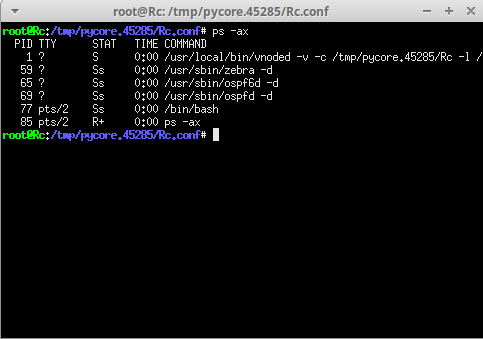
\includegraphics[scale = 0.6]{processos-routerc-ex2b.png}
	\caption{Processos do router}
\end{figure}

\newpage

\begin{figure}[h]
	\centering
	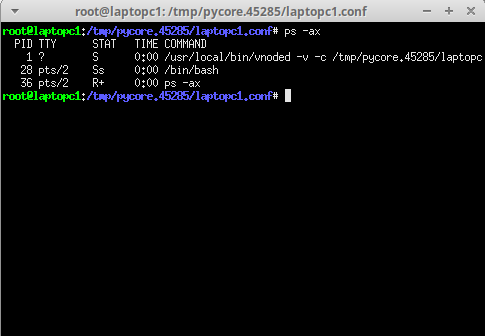
\includegraphics[scale = 0.6]{processos-laptop-ex2b.png}
	\caption{Processos de um laptop}
\end{figure}


\subsubsection{Alinea c}
\textbf{Admita que, por questões administrativas, a rota por defeito (0.0.0.0 ou  default) deve ser retirada definitivamente da tabela de encaminhamento do servidor S1  localizado nodepartamento A. Use o comando route delete para o efeito. Que implicações tem esta medida para os utilizadores da organização MIEI-RC que acedem ao servidor. Justifique.}\\\par
Ao remover a rota por defeito o servidor $S_1$ deixa de conseguir responder a quem não se encontra na sua subrede, apesar de conseguirem aceder ao servidor. Isto acontece, porque apesar de todos os elementos da rede conhecem o servidor $S_1$, este apenas consegue encaminhar mensagens para a sua subrede.\\

\subsubsection{Alinea d}
\textbf{Adicione as rotas estáticas necessárias para restaurar a conectividade para o servidor S1, por forma a contornar a restrição imposta na alínea c). Utilize para o efeito   o comando route add e registe os comandos que usou.}\\\par
Para restabelecer a conectividade para o servidor $S_1$, é necessário adicionar à tabela de encaminhamento do servidor rotas para as três subredes(10.6.0.0, 10.0.7.0, e 10.0.8.0).\par
Os comandos utilizados para restabelecer as rotas foram:
\begin{itemize}
	\item route add -net 10.0.8.0 netmask 255.255.255.0 gw 10.0.5.1
	\item route add -net 10.0.7.0 netmask 255.255.255.0 gw 10.0.5.1
	\item route add -net 10.0.6.0 netmask 255.255.255.0 gw 10.0.5.1
\end{itemize} 

\subsubsection{Alinea e}
\textbf{Teste a nova política de encaminhamento garantindo que o servidor está novamente acessível, utilizando para o efeito o comando ping. Registe a nova tabela de encaminhamento do servidor.}\\\par
Depois de adicionar as novas entradas à tabela de encaminhamento, a conexão foi restabelecida, como podemos ver na imagem.\\

\begin{figure}[h]
	\centering
	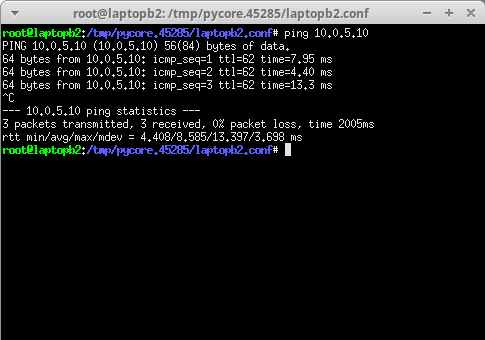
\includegraphics[scale = 0.6]{conectividade-ex2e.png}
	\caption{Teste de conectividade}
\end{figure}

\subsection{Ex3}
\textbf{Por forma a minimizar a falta de endereços IPv4 é comum a utilização de sub-redes. Além disso, a definição de sub-redes permite uma melhor organização do espaço de endereçamento das redes em questão. Para definir endereços de sub-rede é necessário usar a parte prevista para endereçamento de host, não sendo possível alterar o endereço de rede original. Recorda-se que o subnetting, ao recorrer ao espaço de endereçamento para  host, implica que possam ser endereçados menos hosts. Considere a topologia definida   anteriormente. Assuma que o endereçamento entre os routers se mantém inalterado, contudo, o endereçamento em cada departamento deve ser redefinido.}

\newpage

\subsubsection{Alinea 1}
\textbf{Considere que dispõe apenas do endereço de rede IP 130.XX.96.0/19, em que XX é o decimal correspondendo ao seunúmero de grupo (PLXX). Defina um novo esquema   de endereçamento para as redes dos departamentos (mantendo a rede de acesso e core inalteradas) e atribua endereços às interfaces dos vários sistemas envolvidos. Assuma que todos os endereços de sub-redes são usáveis. Deve justificar as opções usadas.}\\\par
Na nossa resolução decidimos usar os 5 bits do terceiro octeto para identificar as nossas subredes e os restantes 8 bits para atribuiçao de ips.
Esta escolha foi feita de forma a premitir crescimento tanto ao nível de subredes como na distribuição de ips, uma vez que no modelo atual, seriam necessários apenas 2 bits para representar as 4 subredes e 3 bits para representar as diferentes interfaces em cada subrede.\par Desta forma, atribuímos os endereços 130.61.96.0 / 24 ao departamento A, 130.61.97.0 / 24 ao departamento B, 130.61.98.0 / 24 ao departamento C, e por fim, 130.61.99.0 / 24 ao departamento D.

\begin{figure}[h]
	\centering
	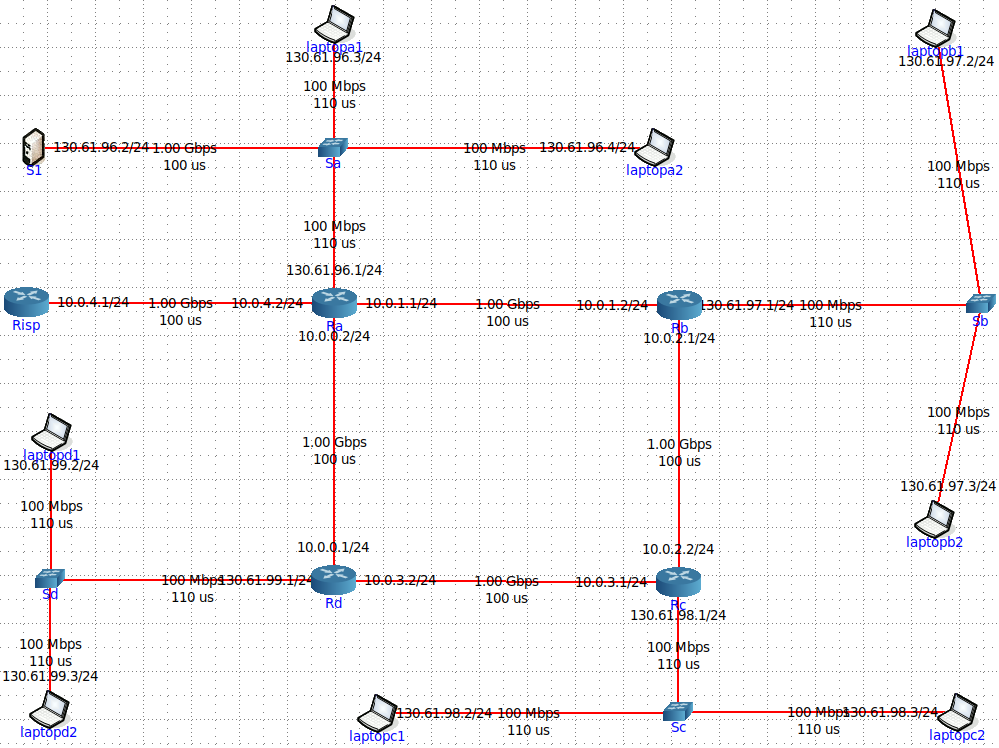
\includegraphics[scale = 0.4]{rede-tp2-ex3.png}
	\caption{Topologia da rede}
\end{figure}

\subsubsection{Alinea 2}
\textbf{Qual a máscara de rede que usou (em formato decimal)? Quantos hosts IP pode interligar em cada departamento? Justifique.}\\\par
A mascara de rede usada foi: 255.255.255.0.\par
Uma vez que os endereços com os bits todos a zero e a um não são usáveis, podemos ligar a $2^8 - 2 = 254$ endereços.

\subsubsection{Alinea 3}
\textbf{Garanta e verifique que conectividade IP entre as várias redes locais da organização MIEI-RC é mantida. Explique como procedeu.}\\\par
Para verificar a conectividade entre as várias redes locais, enviamos pings desde o servidor do departamento A até um laptop de cada departamento. 

\begin{figure}[h]
	\centering
	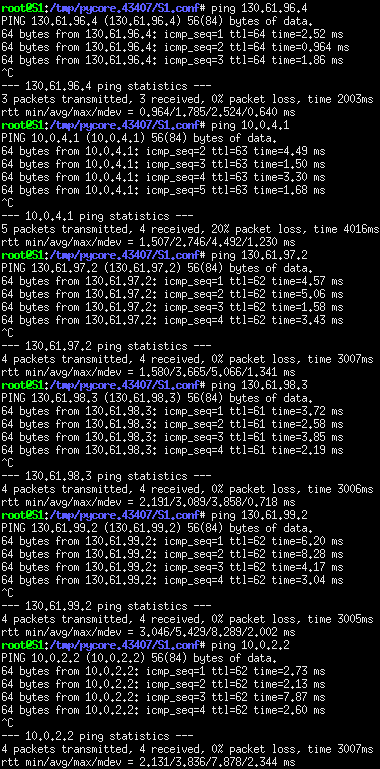
\includegraphics[scale = 0.4]{teste-conectividade-ex3.png}
	\caption{Teste de conectividade}
\end{figure}

\section{Conclusão}

Este trabalho prático serviu de complemento às aulas teóricas e ajudou a consolidar a matéria lecionada nas mesmas.\par
Através da máquina virtual disponibilizada, tivemos a oportunidade de desenvolver as nossas capacidades de construção de Topologias CORE.\par 
Relativamente ao capítulo de IP: Internet Protocol, ficamos a perceber melhor como é que o TTL funciona uma vez que tivemos a oportunidade de analisar vários exemplos, assim como a importância de tentar ter o menor TTL possível, mas que consiga chegar ao destino desejado.\par
Quanto ao formato de um datagrama IP, a par das aulas teóricas, identificamos os dois campos constituintes no datagrama: campo de dados (payload) e cabeçalho.\par
Averiguamos também a fragmentação de datagramas, e consequentemente, fomos confrontados com a importância do campo relativo à fragmentation, com respetivas flags (\texit{reserved bit}, \texit{don't fragment}, \textit{more fragments} e \texit{fragment offset}) (IPv4).\par
Relembramos ainda a definição de endereços públicos e privados e de switches.\par
Analisamos tabelas de encaminhamento e recordamos a definição de encaminhamento estático e dinâmico. Implicitamente, os conceitos de classfull e classless
também foram utilizados.\par
Também trabalhamos com a definição de rotas estáticas e manipulação das mesmas.\par
O conceito de subnetting foi posto à prova com a necessidade da divisão de endereços e a importância das máscaras de rede foi também, mais uma vez, realçada.\par
Resumindo, basicamente todo o capítulo de Protocolo IP foi abrangido e relembrado, e os conceitos inerentes ao mesmo foram consolidados.\par


\printindex
\end{document}
